\subsection{Assembly task} % (fold)
\label{sub:assembly_task}

There are four different types of parts, numbered $1$ through $4$,
which can be combined to form larger parts according to the assembly
plans in Fig. \ref{fig:assembly_plans}. Parts bond together through
bi-directional connections at sites along their perimeters. The last
step in each plan is the production of a final assembly, $F1$ or
$F2$.  The assembly task is executed by a group of robots in an
arena that is sufficiently large to ignore the dynamics of
small-scale interactions.  Initially, robots and many copies of
parts of type $1$ through $4$ are randomly scattered throughout the
arena. There are exactly as many of these parts as are needed to
create a specified number of final assemblies, and the number of
robots equals the total number of scattered parts. Each robot knows
the assembly plans a-priori and has the ability to recognize part
types, pick up a part, combine it with one that is being carried by
another robot, and disassemble a part it is carrying.

Our objective is to define robot controllers for moving around the
arena and for picking up, assembling, and disassembling parts so
that the robots produce target numbers of final assemblies as
quickly as possible.

\begin{figure}[t]
    \centering
        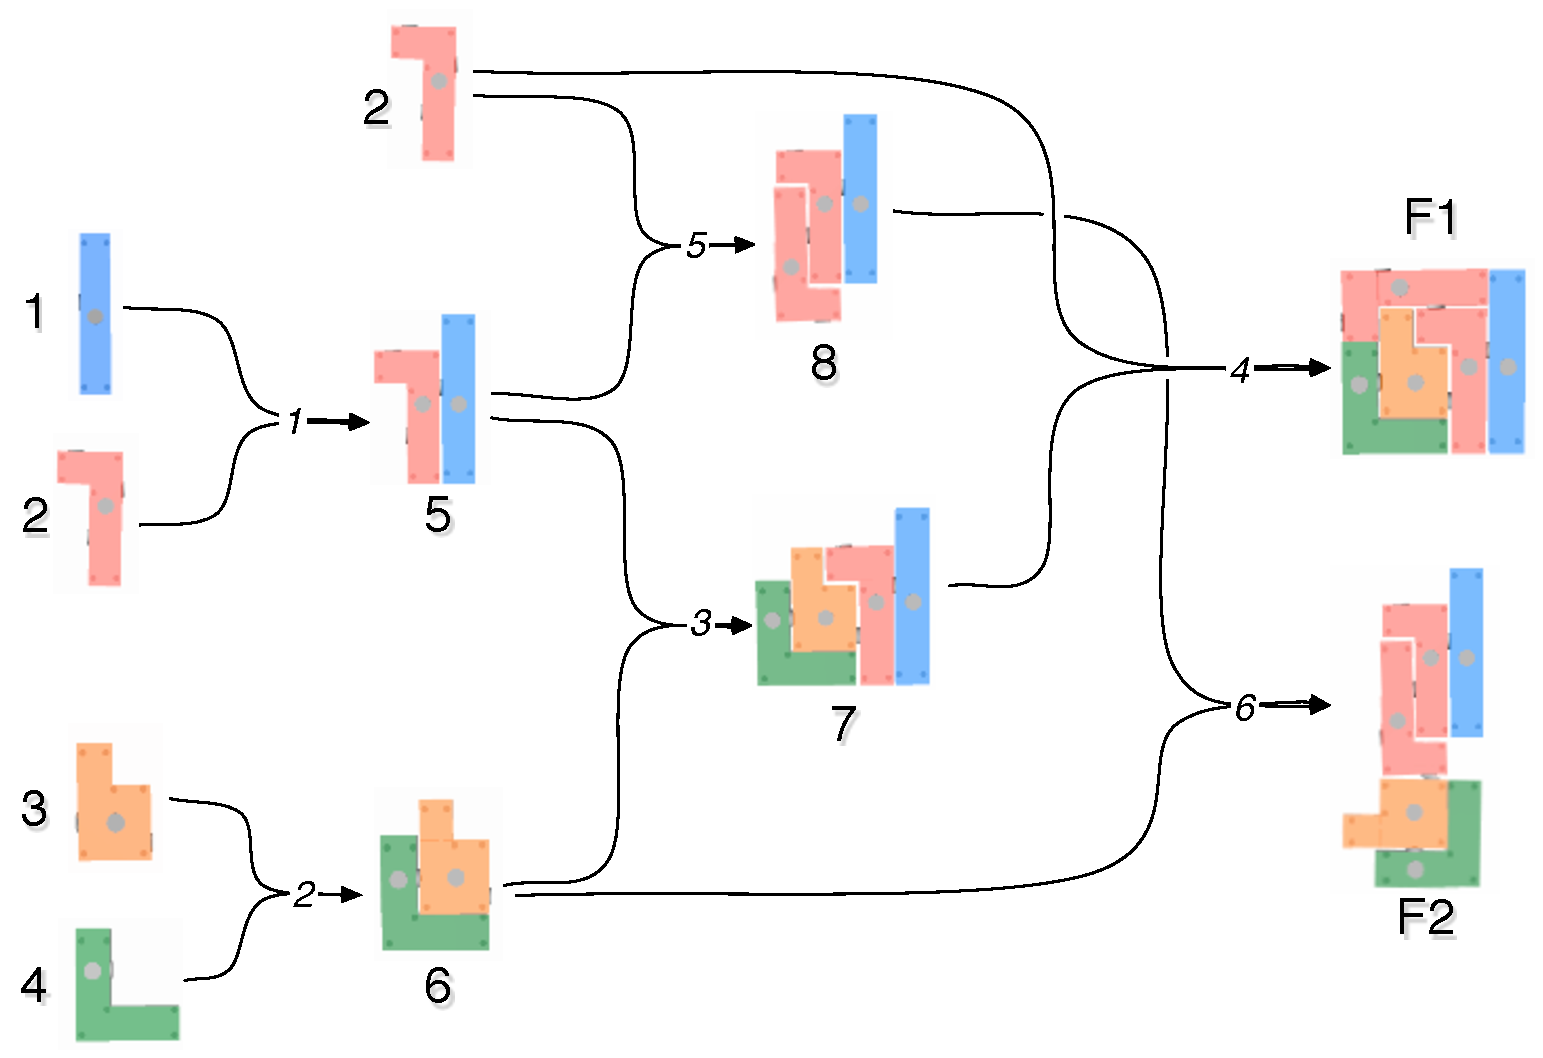
\includegraphics[width=8cm]{img/assembly_plans.pdf}
    \caption{Assembly plans for final assemblies F1 and F2.}
    \label{fig:assembly_plans}
\end{figure}


%, that can be combined into two possible final assemblies, $F1$ and
%$F2$.  Each final assembly is built from components $1, 3, 4$, and
%two copies of $2$ according to the plans in Fig.
%\ref{fig:assembly_plans}.

% subsection assembly_task (end)

\subsection{Micro-continuous model} % (fold)
\label{sub:stochastic_assembly}

We implement the assembly task in the robot simulator Webots
\cite{Michel:2004p10762}, which uses the Open Dynamics Engine to
accurately simulate physics.  We use the robot platform Khepera III,
which has infra-red distance sensors for collision avoidance. Each
robot is outfitted with a protruding bar with a rotational servo at
the tip.  A magnet on the servo bonds to a magnet on the top face of
a part, and the servo is used to rotate the bonded part into the
correct orientation for assembly.  Parts bond to each other via
magnets on their side faces.  Magnets can be turned off to
deactivate a bond.  Robots and parts are equipped with a radio
emitter and receiver for local communication and for computing
relative bearing, which is used to align robot and part magnets and
to rotate a part for assembly. The task takes place inside the
walled hexagonal arena shown in Fig. \ref{fig:overall_arena}.

We use a control policy for the robots that is inspired by chemical
processes: random movement patterns with probabilistic assemblies
upon encounter, as well as random disassemblies.  Our models assume
that the system is well-mixed; to achieve this property, robots move
according to a random walk, and we verify that the space is
uniformly covered. Robots and parts switch between action states
based on information they receive via local sensing and
communication.  When a robot encounters a part on the ground, it
approaches and bonds to it and starts searching for a robot that is
carrying a compatible part, according to the assembly plans.  When
one is found, the two robots align their parts and approach each
other to join the parts.  One robot carries off the newly assembled
part while the other resumes searching for a part on the ground. A
robot can disassemble a part it is carrying by dropping one of the
component parts on the ground.  To control the outcome of part
populations, we can directly modify the probabilities of starting an
assembly and performing a disassembly.

%modify directly the rates of assemblies
%     and disassemblies. More precisely, we control the probabilities of starting an assembly
%     or a disassembly.

 %       We keep track of the populations of pieces and assemblies, for several experiments with
 %   random initial positions of pieces and robots in the arena.

%this is used to align a servo magnet with a part magnet and to
%rotate a part by the necessary angle.

%Robots also use the radio to compute their relative angle to a part,
%which is used to align the servo magnet with the part magnet and to
%rotate the part by the necessary angle.


%The connector at the tip of this arm can rotate freely to align
%components for assembly.

\begin{figure}[t]
\centering
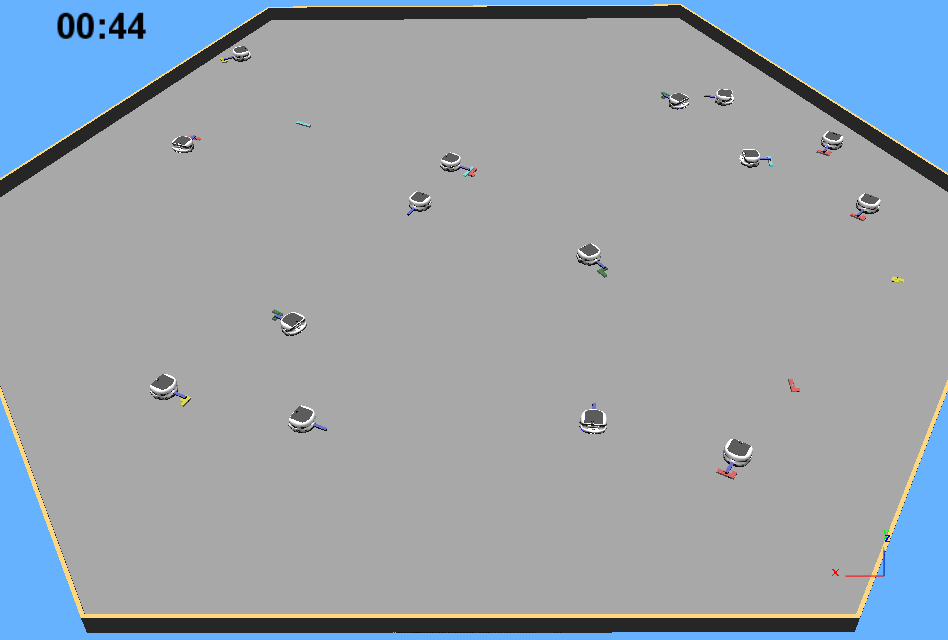
\includegraphics[width=8cm]{img/overall_arena_3.png}
\caption{Snapshot of the arena in the realistic physical simulation.
Robots carry parts at the end of a protruding bar.}
\label{fig:overall_arena}
\end{figure}

% subsection stochastic_assembly (end)